\section{Displej z~tekutých krystalů (LCD)}
Pro zobrazování informací uživateli přímo na~zařízení byl využit alfanumerický\footnote{Alfanumerický -- Řídící jednotka displeji místo pixelů posílá celé znaky, které sám vykresluje.} LCD s řadičem HD44780 a~s rozlišením 20~x~4 znaky. K displeji je~také připojen I$^{2}$C převodník, který slouží jako prostředník mezi řadičem displeje a~Raspberry Pi.
Komunikační protokol LCD totiž využívá podstatně více kontaktů, než I$^{2}$C sběrnice, kterou Raspberry Pi~komunikuje s převodníkem. Převodník je~k pinům Raspberry Pi~připojen dle tabulky~\ref{tab:LCD_conn}.

\begin{figure}[htb]
  \centering
  \begin{minipage}{0.45\textwidth}
    \centering
    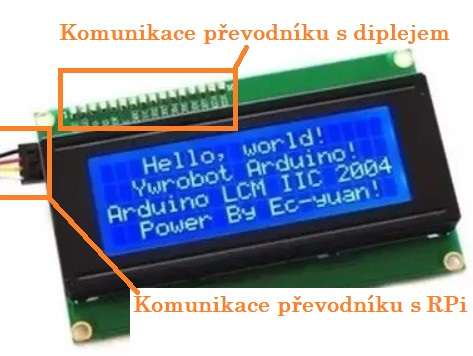
\includegraphics[width=1\textwidth]{img/LCD_front.jpg} % first figure itself
    \caption{\label{fig:LCD_front} Displej z~tekutých krystalů (LCD); Převzato a~upraveno z~\cite{laskakit-LCD}}
  \end{minipage}\hfill
  \begin{minipage}{0.45\textwidth}
    \centering
    \includegraphics[width=1\textwidth]{img/LCD_back.jpg} % second figure itself
    \caption{\label{fig:LCD_back} I$^{2}$C převodník napojený na~LCD~\cite{laskakit-LCD}}
  \end{minipage}
\end{figure}

\begin{table}[htb]
  \centering
  \begin{tabular}{c|c}
    kontakt převodníku & kontakt RPi \\
    \hline
    GND                & GND         \\
    5V                 & 5V          \\
    SCK                & GPIO3       \\
    SDA                & GPIO2       \\
    LED                & GPIO18      \\
  \end{tabular}
  \caption{\label{tab:LCD_conn} Připojení kontaktů I$^{2}$C převodníku na~kontakty RPi.}
\end{table}


\section{Rotační enkodér~\cite{how-encoders-work}\cite{rotary-encoder-cvut}}
Rotační enkodér je~typ pozičního senzoru používaný k měření rotace otáčivé hřídele. Existuje mnoho druhů enkodérů, rozdělují se~dle signálu, který vydávají a~dle technologie, kterou měří rotaci hřídele. V této práci je~použit mechanický inkrementální enkodér s tlačítkem.

Na obrázku~\ref{fig:encoder-working} je~vidět, jak enkodér funguje uvnitř. Dva kontakty A~a B při rotaci získávají a~ztrácí kontakt s kontaktem C. Připojíme-li ke~kontaktu C zem a~ke~kontaktům A~a B pull-up rezistory (klidně softwarově), dá se~toto získávání a~ztrácení kontaktu zaznamenat do~grafu na~obrázku~\ref{fig:encoder-graph} jako dva signály obdélníkového průběhu vzájemně fázově posunuté o 90 stupňů.

\begin{figure}[htb]
  \centering
  \begin{minipage}{0.45\textwidth}
    \centering
    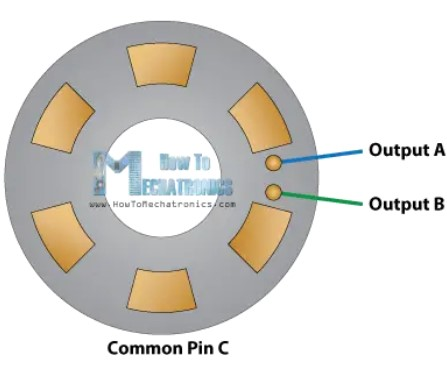
\includegraphics[width=1\textwidth]{img/encoder-working.jpg}
    \caption{\label{fig:encoder-working} Vnitřní schéma enkodéru~\cite{how-encoders-work}}
  \end{minipage}\hfill
  \begin{minipage}{0.45\textwidth}
    \centering
    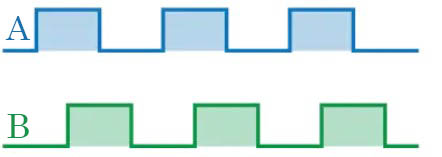
\includegraphics[width=1\textwidth]{img/encoder-graph.jpg}
    \caption{\label{fig:encoder-graph} Výstup enkodéru~\cite{how-encoders-work}}
  \end{minipage}
\end{figure}

Použitý rotační enkodér má další dva kontakty připojené k tlačítku pod rotující hřídelí. Ke~čtení stisknutí tlačítka je~potřeba připojit jeden kontakt k zemi, tedy ke~kontaktu C a~druhý kontakt na~pull-up rezistor (klidně softwarově). Celé zapojení enkodéru je~naznačeno na~obrázku~\ref{fig:encoder-pinout}. Kontakty tlačítka jsou v něm označeny S1 a~S2. Enkodér je~k RPi připojen dle tabulky~\ref{tab:enc_conn}.

\begin{table}[htb]
  \centering
  \begin{tabular}{c | c}
    kontakt enkodéru & kontakt RPi \\
    \hline
    C                & GND         \\
    S2               & GND         \\
    A~               & GPIO5       \\
    SDA              & GPIO6       \\
    S1               & GPIO13      \\
  \end{tabular}
  \caption{\label{tab:enc_conn} Připojení kontaktů rotačního enkodéru na~kontakty RPi.}
\end{table}


\subsection{Čtení pozice z~rotačního enkodéru}
U rotačního enkodéru se~při každé otáčce změní připojení pinů několikkrát. Chceme-li pozorovat pouze počet těchto změn, stačí spočítat změny na~jednom kontaktu. Pokud je~ale zapotřebí pozorovat i směr otáčení, je~nutné pozorovat stav obou kontaktů. Pokud se~enkodér otáčí po~směru hodinových ručiček, kontakt A~bude fázově posunut o 90 stupňů napřed oproti kontaktu B.
Pokud se~eknodér otáčí proti směru hodinových ručiček, bude naopak kontakt B o 90 stupňů napřed oproti kontaktu A. Časový průběh stavu kontaktů je naznačen na obrázku~\ref{fig:encoder_data}.
\begin{figure}[htb]
  \centering
  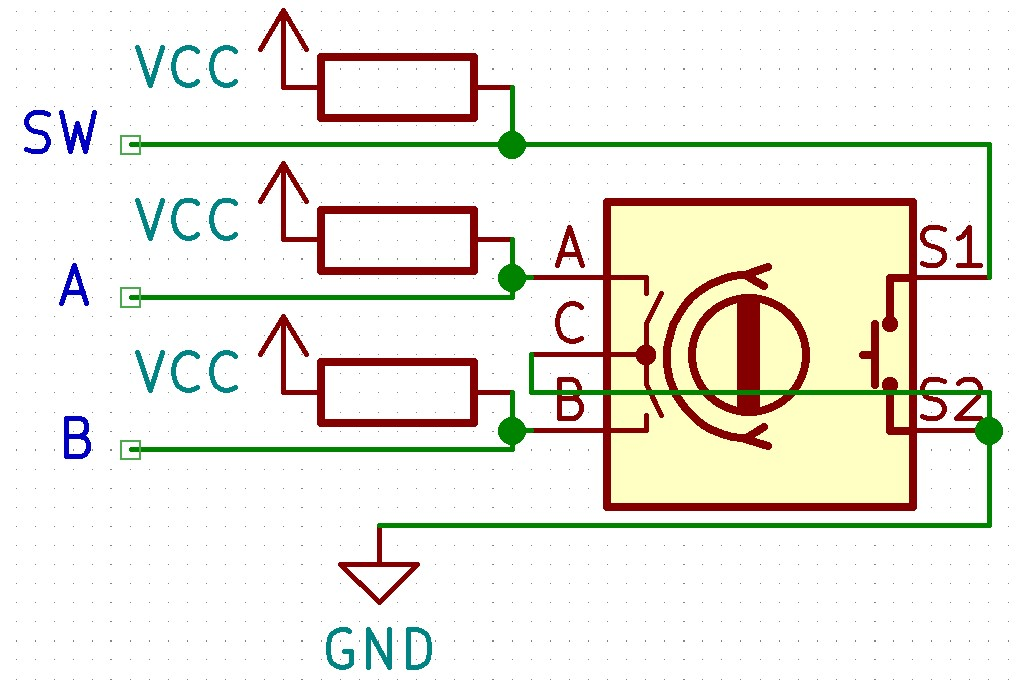
\includegraphics[width=0.5\textwidth]{img/encoder-pinout.jpg}
  \caption{\label{fig:encoder-pinout} Schéma zapojení rotačního enkodéru.}
\end{figure}
\begin{figure}[htb]
  \centering
  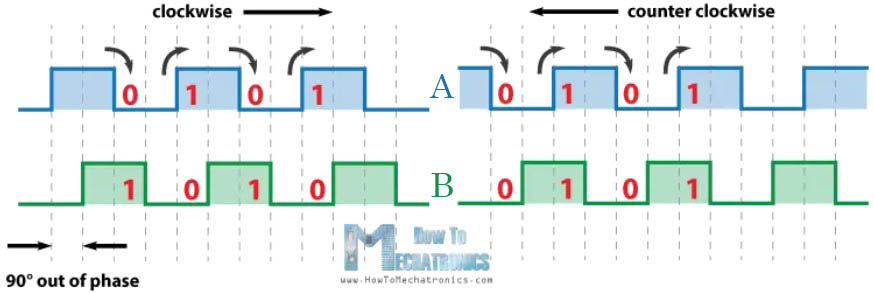
\includegraphics[width=1\textwidth]{img/encoder_data.jpg}
  \centering
  \caption{\label{fig:encoder_data} Časový průběh stavu kontaktů rotačního enkodéru při otáčení hřídelí na obě strany}
\end{figure}
